\begin{figure}[!ht]
	\centering
    \makebox[\textwidth][c]{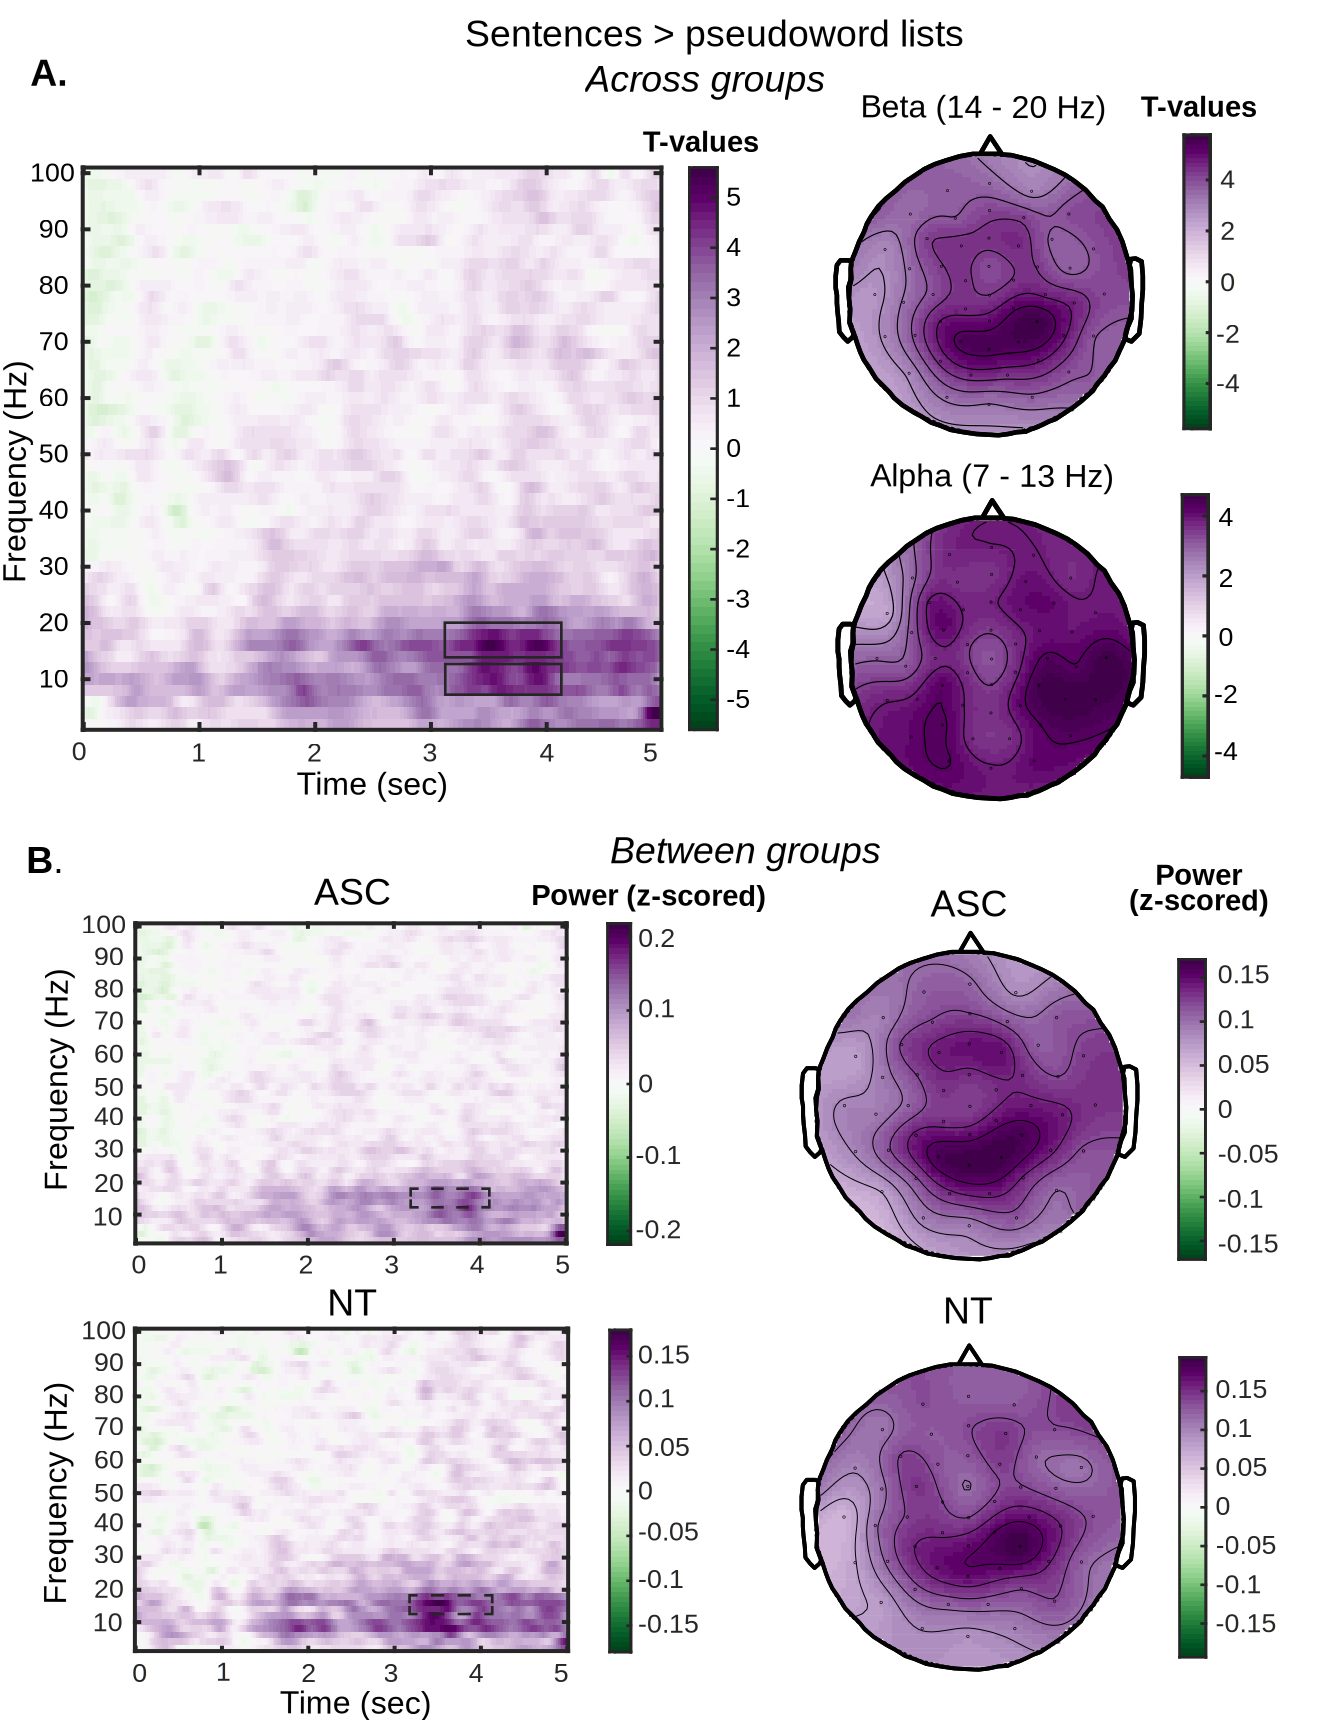
\includegraphics[width=.8\textwidth]{./Chapters/04_LanguageASC/Images/TFSpectrumFull_vert.eps}}
	\caption{Time-frequency (TF) dynamics in Sentences vs. pseudoword list contrast. (a) TF power is significantly different for the contrast, with power differences present across almost all channels, frequencies and timepoints. The color scale shows the relative difference in TF power (0 = no change). The timepoints and frequencies where the effect is strongest are indicated with boxes on the left, and the corresponding topography on the right for two different frequency bands: 14 - 20 Hz (beta) with bilateral posterior peaks, and 7 - 13 Hz (alpha) with a more widespread spatial effect. (b) TF power for the contrast was not different between neurotypical (NT) and autistic (ASC) participants. On the left, the similar TF spectra are shown, with the rectangle indicating the strongest power changes and on the right, the topography of this effect. }
    \vspace*{-10pt}
	\label{fig:tf-spectrum-full}
\end{figure}


